\documentclass[conference]{IEEEtran}

\usepackage[T1]{fontenc}
\usepackage[utf8]{inputenc}
\usepackage{amsmath,amssymb}
\usepackage{booktabs}
\usepackage{array}
\usepackage{graphicx}
\usepackage{xcolor}
\usepackage{tikz}
\usetikzlibrary{arrows.meta,positioning,patterns,calc}
\usepackage{url}
\usepackage[hidelinks]{hyperref}
\usepackage{cite}
\usepackage{microtype}
\usepackage{dblfloatfix}
\usepackage{balance}
\usepackage{capt-of}

\setcounter{topnumber}{4}
\setcounter{dbltopnumber}{3}
\renewcommand{\topfraction}{0.95}
\renewcommand{\dbltopfraction}{0.95}
\renewcommand{\textfraction}{0.05}
\renewcommand{\floatpagefraction}{0.85}
\renewcommand{\dblfloatpagefraction}{0.85}

\definecolor{oiOrange}{HTML}{E69F00}
\definecolor{oiSkyBlue}{HTML}{56B4E9}
\definecolor{oiBluishGreen}{HTML}{009E73}
\definecolor{oiYellow}{HTML}{F0E442}
\definecolor{oiBlue}{HTML}{0072B2}
\definecolor{oiVermillion}{HTML}{D55E00}
\definecolor{oiReddishPurple}{HTML}{CC79A7}
\definecolor{softGray}{HTML}{666666}

\title{FLOMAP: Rectified-Flow Guidance with CS-PIBT Collision Shielding for Multi-Agent Path Finding\\[0.25em]
{\large Spring 2026 Research Report}}

\author{
\IEEEauthorblockN{
\begin{tabular}{@{}c@{}}
\begin{tabular}{c}
Barathkrishna Satheeshkumar\\
Carnegie Mellon University\\
\texttt{bsathees@andrew.cmu.edu}
\end{tabular}
\\[0.9em]
\begin{tabular}{@{}c@{\hspace{3.5em}}c@{}}
\begin{tabular}{c}
Maxim Likhachev\\
Advisor, Carnegie Mellon University\\
\texttt{maxim@cs.cmu.edu}
\end{tabular}
&
\begin{tabular}{c}
Matthew Travers\\
Advisor, Carnegie Mellon University\\
\texttt{mtravers@andrew.cmu.edu}
\end{tabular}
\end{tabular}
\end{tabular}
}
}

\begin{document}
\maketitle

\begin{abstract}
Learning-based multi-agent path finding (MAPF) is attractive because neural
policies can scale to large agent populations and can learn structural
regularities from data.  However, many shielded learned MAPF systems, including
discrete action classifiers such as SSIL, make one-step action predictions that
may remain myopic in dense or bottlenecked coordination regimes.  This report
studies FLOMAP, a CS-PIBT-shielded policy that aims to provide smoother
directional guidance via a continuous rectified-flow velocity representation
rather than directly predicting discrete grid actions.  The learned velocity is
converted into ranked action preferences and executed through the same CS-PIBT
collision shield used by the baselines.  We test whether this continuous
flow-based guidance can improve over discrete learned actions or heuristic
shortest-path preferences under a shared shielded interface.  On the primary
held-out evaluation, FLOMAP
reaches 64.59\% all-agent success compared with 66.43\% for SSIL, and the
difference on non-coordination-heavy slices is not significant under a paired
McNemar test ($p=1.0$).  The
gap is concentrated on dense random and maze bottleneck maps.  A shared-shield
comparison further shows that BD-PIBT, a non-learned backward-Dijkstra
preference baseline, achieves the best performance in this evaluation:
it ties SSIL on the primary evaluation and reaches 59.48\% on the extended
topology evaluation, compared with 55.22\% for SSIL and 53.07\% for FLOMAP.  The
main contribution is a controlled diagnostic evaluation of continuous flow
guidance for MAPF: it shows what learned velocity fields capture, where
coordination topologies remain challenging, and why backward-Dijkstra
preferences with CS-PIBT constitute a strong baseline that learned shielded MAPF
policies must surpass.
\end{abstract}

\section{Introduction}

Multi-agent path finding requires a set of agents to move from distinct starts to
distinct goals on a shared graph without vertex or edge collisions.  The problem
is computationally difficult at large scale, yet practical MAPF systems often
need to make decisions repeatedly for hundreds or thousands of agents.  Classical
search methods such as CBS and EECBS provide strong solution-quality guarantees
or bounded suboptimality, but they can be too expensive for the largest
interactive settings \cite{sharon2015cbs,li2021eecbs}.  Reactive and prioritized
methods such as PIBT scale much better, but their one-step decisions may fail
to resolve narrow bottlenecks or dense coordination patterns
\cite{okumura2019pibt}.

We investigate whether continuous flow-based guidance can outperform one-step
discrete action policies or heuristic shortest-path preferences when all
methods are executed through the same collision-shield interface.

The SSIL line of work showed that a simple graph neural classifier, when wrapped
in a CS-PIBT collision shield, is a strong learned MAPF baseline
\cite{veerapaneni2025wsnh}.  SSIL predicts one of five discrete
actions: wait, right, down, up, or left.  FLOMAP studies a different
interface: instead of directly predicting a discrete action distribution, a
rectified-flow GNN predicts a continuous 2D velocity vector.  The
velocity direction induces action preferences, the velocity magnitude helps
identify states where waiting is appropriate, and CS-PIBT remains responsible
for one-step collision avoidance.

We also evaluate a non-learned BD-guided CS-PIBT baseline.
This comparison is necessary because CS-PIBT can already consume strong
shortest-path preferences without a neural policy.  A fair learned-guidance
study must therefore ask whether the learned preference generator improves over
the heuristic preferences available to the same shield, not only whether it is
close to another learned classifier.  In this shared protocol, FLOMAP trails
SSIL on the primary evaluation under a paired McNemar test ($p=0.0039$), but
the non-stress learned-policy slices are not significantly different
($p=1.0$); BD-PIBT achieves the best performance in this evaluation.  The
action-head, hybrid, and
coordination-focused data
ablations are interpreted as evidence about design trade-offs rather than as
separate final methods.

This report makes three contributions.  First, it introduces a continuous-velocity
policy interface for shielded MAPF in which a rectified-flow GNN predicts
continuous guidance before discrete action ranking.  Second, it provides a
controlled comparison between learned and heuristic preference generators under
identical CS-PIBT execution, showing that backward-Dijkstra preferences combined
with CS-PIBT form a strong baseline that learned policies must surpass.  Third,
it reveals topology-dependent failure modes of learned
policies, showing when learned velocity guidance is close to SSIL and when dense or
bottlenecked maps expose remaining weaknesses.

\section{Background and Related Work}

\subsection{MAPF and Collision Shielding}

CBS is the canonical optimal two-level MAPF solver, resolving conflicts by
branching over constraints while solving single-agent paths at the low level
\cite{sharon2015cbs}.  EECBS adds explicit estimation and focal search to obtain
bounded-suboptimal solutions more efficiently \cite{li2021eecbs}.  These solvers
are important as expert data generators and reference planners, but the online
cost can grow rapidly with agent count and conflict density.

PIBT is an iterative MAPF method that assigns dynamic priorities and uses
priority inheritance with backtracking to resolve one-step conflicts
\cite{okumura2019pibt}.  LaCAM extends search-based MAPF with lazy constraint
addition and is relevant as a stronger lookahead direction for future shielded
policies \cite{okumura2023lacam}.  CS-PIBT, used by SSIL and this work,
retains the PIBT-style one-step collision-resolution mechanism but consumes an
external action-preference ordering \cite{veerapaneni2025wsnh}.  The preference
generator may be learned, as in SSIL and FLOMAP, or heuristic, as in a
backward-Dijkstra distance-to-goal ranking.  This separation is useful for
evaluation: the policy supplies preferences, while the shield prevents immediate
vertex and edge collisions.  It also means that BD-guided CS-PIBT is a strong
classical baseline under the same execution interface.

\subsection{Learning-Based MAPF}

SSIL is the learned classifier baseline because it uses the same shielded
evaluation interface and a lightweight GNN policy trained from EECBS
demonstrations \cite{veerapaneni2025wsnh}.  Its architecture is aligned with
the action space used by CS-PIBT: node features include neighborhood image
patches and backward-Dijkstra heuristics, the graph trunk uses GraphSAGE
message passing, and the output is a five-way action classifier.  This alignment
is important for interpretation.  If a map requires precise waiting or yielding,
SSIL receives direct supervision on the same discrete decision that the shield
later consumes.  BD-PIBT provides a complementary non-learned baseline: it uses
the same shield but replaces the neural preference generator with a
distance-to-goal action ordering.

FLOMAP uses the same broad shielded-imitation setting but replaces the
primary output with a continuous velocity vector.  The trunk uses GraphSAGE
aggregation \cite{hamilton2017graphsage} implemented with PyTorch Geometric
\cite{fey2019pyg}.  This introduces a different inductive bias: the model can
represent smooth neighborhood motion fields, but the final interface must still convert
those fields to five discrete actions.

\subsection{Flow-Based Policies}

Rectified Flow learns an ordinary differential equation that transports samples
between a base distribution and a data distribution along approximately linear
interpolation paths \cite{liu2023rectifiedflow}.  Flow Matching and Conditional Flow Matching
provide related simulation-free objectives for continuous normalizing flows
\cite{lipman2023flowmatching,tong2024cfm}.  In robotics, generative policies
such as Diffusion Policy motivate continuous or distributional action-generation
interfaces for control \cite{chi2023diffusionpolicy}.  The FLOMAP setting
differs from continuous robot control because execution remains restricted to
discrete grid moves.  The flow model therefore acts as a continuous preference
generator for a discrete collision shield.

\section{Problem Formulation}

Let $\mathcal{G}=(V,E)$ be a four-connected grid graph with static obstacles.  A
MAPF instance contains $N$ agents with starts
$\mathbf{s}=(s_1,\ldots,s_N)$ and goals $\mathbf{g}=(g_1,\ldots,g_N)$, where
$s_i,g_i\in V$.  At time step $t$, agent $i$ occupies $v_i^t$ and chooses an
action from
\[
\mathcal{A}=\{\mathrm{wait},\mathrm{right},\mathrm{down},\mathrm{up},\mathrm{left}\}.
\]
A valid execution avoids vertex conflicts,
$v_i^t\neq v_j^t$ for all $i\neq j$, and edge-swap conflicts,
$(v_i^t,v_i^{t+1})\neq(v_j^{t+1},v_j^t)$.  The primary evaluation metric is
all-agent success: a run succeeds only if every agent reaches its
goal within the step and time limits.  The secondary metric is the mean fraction
of agents at goal, which distinguishes complete failures from near-completions.

We formulate learning as imitation under shielding.  Given an expert trajectory,
the model observes neighborhood grid information, heuristic features, and
nearby-agent interactions.  It outputs either a continuous velocity vector
$\hat{\mathbf{v}}_i\in\mathbb{R}^2$ or, in ablation modes, discrete action
logits.  CS-PIBT then selects collision-free actions from the induced preference
lists.  The shield guarantees one-step collision avoidance for the selected
time step, but it does not guarantee global progress to the goal under arbitrary
preferences.

\section{Method}

\subsection{MAPF with CS-PIBT}

FLOMAP retains CS-PIBT as a collision shield.  At each simulation step, the
learned model produces an action-preference list for every agent.  CS-PIBT then
applies priority inheritance and backtracking to resolve one-step conflicts and
returns a legal joint move.  This separation prevents the learned policy's
preferences from directly producing illegal one-step moves, while preserving the
policy's influence over which legal moves are attempted first.

\subsection{Rectified-Flow Objective}

For each agent time step sample, let $\mathbf{x}_1$ be the expert velocity vector
derived from the expert grid trajectory and let
$\mathbf{x}_0\sim\mathcal{N}(0,I)$ be Gaussian noise.  Rectified-flow training
samples a time $t\in[0,1]$, constructs an interpolation state, and trains the
flow head with the target vector field:
\begin{align}
\mathbf{x}_t
&=(1-t)\mathbf{x}_0+t\mathbf{x}_1, \\
\mathbf{u}^\star
&=\mathbf{x}_1-\mathbf{x}_0, \\
\mathcal{L}_{\mathrm{flow}}
&=\mathbb{E}\left[w_i\left\|
\hat{\mathbf{u}}_\theta(\mathbf{x}_t,t,\mathcal{G})-\mathbf{u}^\star
\right\|_2^2\right].
\end{align}
The training pipeline supports an auxiliary action cross-entropy loss; however,
the primary FLOMAP model relies exclusively on the flow head during inference.  Ablations
vary the action-loss weight, train action heads on different forward states, or
set the action loss to zero for strict flow-only coordination-data controls.

\subsection{Model Architecture}

A three-layer convolutional encoder processes a neighborhood patch with
obstacle, agent, and goal channels.  The resulting
visual features are concatenated with a five-dimensional backward-Dijkstra
heuristic feature vector and projected to the hidden dimension.  The flow
variables $(\mathbf{x}_t,t)$ are appended before a stack of GraphSAGE layers with
LayerNorm, SiLU activations, and residual connections.  The primary head maps
the shared GNN representation to a 2D flow vector.  An auxiliary
action head maps the same representation to five action logits.

The primary FLOMAP model uses a field-of-view radius $k=4$, a nearby-agent
graph parameter $m=5$, hidden dimension 1024, and six GraphSAGE layers.  Training
uses AdamW with learning rate $10^{-4}$, weight decay $10^{-4}$, cosine learning
rate decay to $10^{-6}$, gradient clipping at 1.0, batch size 256, and a 95/5
train/validation split.
The selected model is trained for up to 20 epochs with validation-based model
selection.  At inference, the flow field is integrated with three Euler steps
and three consensus samples before action ranking.

\begin{figure*}[!tbp]
\centering
\resizebox{0.96\textwidth}{!}{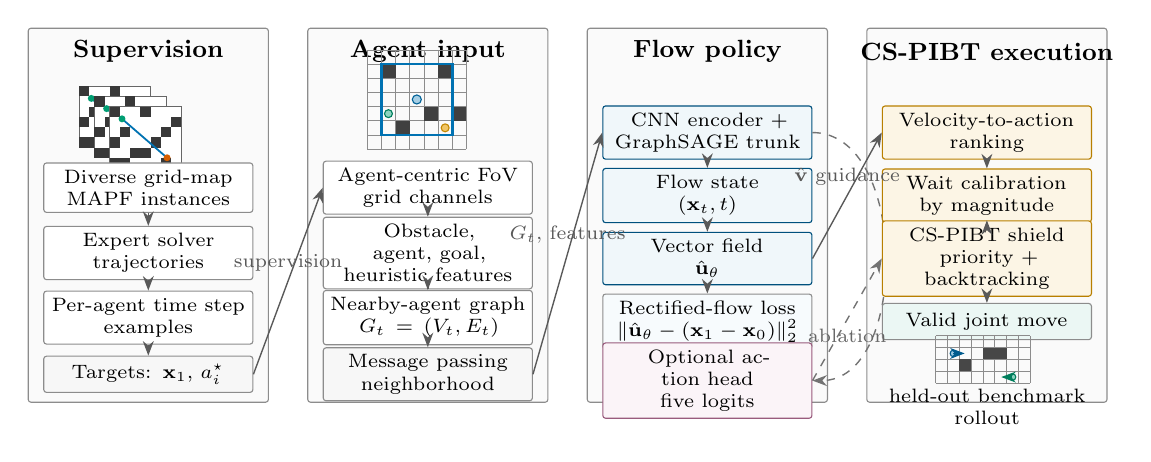
\begin{tikzpicture}[
  font=\scriptsize,
  x=1cm,
  y=1cm,
  stage/.style={
    rectangle,
    draw=black!45,
    fill=black!2,
    rounded corners=1pt,
    minimum width=3.05cm,
    minimum height=4.75cm,
    inner sep=0pt
  },
  title/.style={font=\bfseries\small,align=center},
  box/.style={
    rectangle,
    draw=black!45,
    fill=white,
    rounded corners=1pt,
    align=center,
    text width=2.48cm,
    minimum height=0.46cm,
    inner sep=2.5pt
  },
  bluebox/.style={box,draw=oiBlue!70!black,fill=oiBlue!6},
  orangebox/.style={box,draw=oiOrange!80!black,fill=oiOrange!10},
  purplebox/.style={box,draw=oiReddishPurple!75!black,fill=oiReddishPurple!8},
  arrow/.style={-Stealth,draw=black!65,line width=0.5pt},
  auxarrow/.style={-Stealth,draw=black!55,line width=0.5pt,dashed}
]

% Stage containers.
\node[stage] (supervision) at (0,0) {};
\node[stage] (repr) at (3.55,0) {};
\node[stage] (policy) at (7.10,0) {};
\node[stage] (exec) at (10.65,0) {};

\node[title] at (0,2.08) {Supervision};
\node[title] at (3.55,2.08) {Agent input};
\node[title] at (7.10,2.08) {Flow policy};
\node[title] at (10.65,2.08) {CS-PIBT execution};

% Supervision stage.
\begin{scope}[shift={(-0.88,0.86)},scale=0.13]
  \foreach \dx/\dy in {0/0,1.5/-1.0,3.0/-2.0} {
    \draw[fill=white,draw=black!60,line width=0.35pt] (\dx,\dy) rectangle +(7,6);
    \foreach \x/\y in {0/0,1/0,5/0,2/1,3/1,0/2,4/2,1/3,5/3,6/4,0/5,3/5} {
      \fill[black!78] (\dx+\x,\dy+\y) rectangle +(1,1);
    }
    \draw[oiBlue,line width=0.65pt] (\dx+1.2,\dy+4.8) -- (\dx+5.6,\dy+1.0);
    \fill[oiBluishGreen] (\dx+1.2,\dy+4.8) circle[radius=0.34];
    \fill[oiVermillion] (\dx+5.6,\dy+1.0) circle[radius=0.34];
  }
\end{scope}
\node[box] (maps) at (0,0.35) {Diverse grid-map\\MAPF instances};
\node[box] (solver) at (0,-0.48) {Expert solver\\trajectories};
\node[box] (samples) at (0,-1.30) {Per-agent time step\\examples};
\node[box,fill=black!3] (targets) at (0,-2.02) {Targets: $\mathbf{x}_1$, $a_i^\star$};
\draw[arrow] (maps) -- (solver);
\draw[arrow] (solver) -- (samples);
\draw[arrow] (samples) -- (targets);

% Agent-input stage.
\begin{scope}[shift={(2.78,0.84)},scale=0.18]
  \draw[step=1,black!45,line width=0.25pt] (0,0) grid (7,7);
  \foreach \x/\y in {2/1,4/2,1/5,5/5,6/2} {
    \fill[black!75] (\x,\y) rectangle +(1,1);
  }
  \draw[oiBlue,line width=0.95pt] (1,1) rectangle (6,6);
  \fill[oiBlue!35,draw=oiBlue!85!black] (3.5,3.5) circle[radius=0.32];
  \fill[oiBluishGreen!45,draw=oiBluishGreen!80!black] (1.5,2.5) circle[radius=0.28];
  \fill[oiOrange!60,draw=oiOrange!85!black] (5.5,1.5) circle[radius=0.28];
\end{scope}
\node[box] (fov) at (3.55,0.35) {Agent-centric FoV\\grid channels};
\node[box] (feat) at (3.55,-0.48) {Obstacle, agent, goal,\\heuristic features};
\node[box] (graph) at (3.55,-1.30) {Nearby-agent graph\\$G_t=(V_t,E_t)$};
\node[box,fill=black!3] (msg) at (3.55,-2.02) {Message passing\\neighborhood};
\draw[arrow] (fov) -- (feat);
\draw[arrow] (feat) -- (graph);
\draw[arrow] (graph) -- (msg);

% Policy stage.
\node[bluebox] (trunk) at (7.10,1.05) {CNN encoder +\\GraphSAGE trunk};
\node[bluebox] (state) at (7.10,0.25) {Flow state\\$(\mathbf{x}_t,t)$};
\node[bluebox] (field) at (7.10,-0.55) {Vector field\\$\hat{\mathbf{u}}_\theta$};
\node[box,fill=oiBlue!3] (loss) at (7.10,-1.35) {Rectified-flow loss\\$\|\hat{\mathbf{u}}_\theta-(\mathbf{x}_1-\mathbf{x}_0)\|_2^2$};
\node[purplebox] (action) at (7.10,-2.10) {Optional action head\\five logits};
\draw[arrow] (trunk) -- (state);
\draw[arrow] (state) -- (field);
\draw[arrow] (field) -- (loss);
\draw[auxarrow] (trunk.east) to[out=0,in=0] (action.east);

% Execution stage.
\node[orangebox] (rank) at (10.65,1.05) {Velocity-to-action\\ranking};
\node[orangebox] (wait) at (10.65,0.25) {Wait calibration\\by magnitude};
\node[orangebox] (shield) at (10.65,-0.55) {CS-PIBT shield\\priority + backtracking};
\node[box,fill=oiBluishGreen!8] (move) at (10.65,-1.35) {Valid joint move};
\begin{scope}[shift={(10.00,-2.13)},scale=0.15]
  \draw[step=1,black!45,line width=0.25pt] (0,0) grid (8,4);
  \foreach \x/\y in {2/1,4/2,5/2} {
    \fill[black!72] (\x,\y) rectangle +(1,1);
  }
  \fill[oiBlue!40,draw=oiBlue!80!black] (1.5,2.5) circle[radius=0.28];
  \fill[oiBluishGreen!45,draw=oiBluishGreen!80!black] (6.5,0.5) circle[radius=0.28];
  \draw[arrow,oiBlue!80!black] (1.5,2.5) -- (2.45,2.5);
  \draw[arrow,oiBluishGreen!80!black] (6.5,0.5) -- (5.55,0.5);
\end{scope}
\node[align=center,text width=2.55cm] at (10.65,-2.43) {held-out benchmark\\rollout};
\draw[arrow] (rank) -- (wait);
\draw[arrow] (wait) -- (shield);
\draw[arrow] (shield) -- (move);

% Inter-stage flow.  Keep arrows centered to avoid text collisions.
\draw[arrow] (targets.east) -- node[above,font=\scriptsize,black!65] {supervision} (fov.west);
\draw[arrow] (msg.east) -- node[above,font=\scriptsize,black!65] {$G_t$, features} (trunk.west);
\draw[arrow] (field.east) -- node[above,font=\scriptsize,black!65] {$\hat{\mathbf{v}}$ guidance} (rank.west);
\draw[auxarrow] (action.east) -- node[below,font=\scriptsize,black!60] {ablation} (shield.west);

\end{tikzpicture}
}
\caption{FLOMAP training and execution pipeline.  Expert trajectories on
diverse grid-map MAPF instances are converted into per-agent, per-step
supervision.  The policy input combines an agent-centric field of view with
nearby-agent graph features, which are processed by a CNN encoder and GraphSAGE
message-passing trunk.  The primary branch trains a rectified-flow vector field
and converts the predicted velocity into ranked grid-action preferences; the
dashed branch denotes the auxiliary action-head ablation.  During execution,
CS-PIBT consumes the learned preferences, resolves one-step conflicts through
priority inheritance and backtracking, and outputs valid joint moves for
held-out benchmark rollouts.}
\label{fig:architecture}
\end{figure*}

\subsection{Training Data}

Training samples are generated from EECBS expert trajectories and converted to
per-step graph records.  Expert velocity targets are derived from smoothed
discrete trajectories, while auxiliary action labels are the exact next grid
move from consecutive integer positions.  Each record contains neighborhood
visual context, heuristic features, graph edges between nearby agents, and the
expert velocity or action label.  The primary FLOMAP model is trained on the base
demonstration pool.  The coordination-data ablation uses a targeted
dataset with dense and bottlenecked examples to keep preprocessing tractable
while probing whether additional coordination-heavy demonstrations improve the
observed stress-map behavior.

\subsection{Velocity-to-Action Conversion and Wait Threshold}

FLOMAP integrates the learned vector field for a small number of
Euler steps and averages multiple consensus samples.  The resulting velocity
vector is converted to action scores by dot product with the five grid-action
vectors.  This projection is a simple way to preserve angular alignment between
the continuous velocity and the discrete grid moves consumed by CS-PIBT.  Since
the wait vector is zero, a pure dot-product interface would never naturally
prefer wait.  The implementation therefore applies a fixed wait threshold of
0.25 at inference: if the predicted velocity magnitude is below this value, the
wait action is assigned high probability before CS-PIBT constructs the
preference list.  This threshold is an important part of the flow-to-shield
interface and is a likely bottleneck on maps that require precise waiting.  The
threshold was chosen as a fixed validation-time interface parameter and is not
claimed to be optimal across all topologies.

\subsection{BD-PIBT Baseline}

BD-PIBT is the non-learned classical baseline in this study.  It ranks each
grid action by backward-Dijkstra distance-to-goal preference, with randomized
tie-breaking, and passes the resulting preference lists through the same
CS-PIBT shield used by the learned policies.  At-goal agents prioritize wait,
and invalid moves are deprioritized before shielding.  BD-PIBT uses no neural
model and no GPU; it differs from the learned methods only in the preference
generator supplied to CS-PIBT.  It is therefore not an external solver evaluated
under a different protocol, but the same simulator and shielded execution path
with heuristic action preferences.

\section{Experimental Setup}

\subsection{Benchmarks}

The primary held-out evaluation set is used for the main FLOMAP versus
SSIL comparison.  It contains city, game, open, maze, random-obstacle, and
warehouse-style maps, including both well-connected layouts and topologies with
dense or bottlenecked coordination demands.  The extended topology evaluation
adds maps chosen to expose the model to a broader range of structural patterns,
including both familiar and less familiar map families.

Unless otherwise stated, evaluations use CS-PIBT, a 120 s time limit, a
\texttt{3x} maximum-step multiplier, and a fixed scenario and agent-count
ladder.  BD-PIBT, SSIL, FLOMAP, and the action-head variant are therefore
compared under the same maps, scenarios, agent counts, time limits, and
collision shield.  FLOMAP inference uses three integration steps, three
consensus samples, temperature 0.3, and wait threshold 0.25.  Non-default
action-head models are evaluated with their matching hidden dimension, layer
count, and action-head conditioning.

All compared methods receive goal information through backward-Dijkstra
distance-to-goal features or preferences.  The learned policies receive
agent-centric grid observations, nearby-agent graph connectivity, and
backward-Dijkstra heuristic features, then output learned action preferences.
BD-PIBT receives the same map, start, goal, and backward-Dijkstra information,
but uses the distances directly to rank actions and does not use a neural model.
The learned models receive backward-Dijkstra distances as input features but
must learn to map them to action preferences, whereas BD-PIBT directly uses
these distances to rank actions.  Thus, BD-PIBT represents a strong heuristic
baseline under this interface, while still being evaluated through the same
shielded simulator rather than a different solver interface.

\subsection{Metrics}

The primary metric is all-agent success.  We also include mean agents at
goal, path cost per agent, and average solution time.  Path cost is computed
from the simulator's \texttt{total\_cost\_not\_resting\_at\_goal} column divided
by the number of agents.  Success and agents at goal measure completion and
partial progress, while path cost characterizes efficiency among the shielded
policies.

Runtime is reported as simulator wall-clock time.  BD-PIBT runs without a neural
model or GPU.  Learned policies use neural forward passes and GPU acceleration
when available, so runtime comparisons should be interpreted as implemented
system costs rather than hardware-normalized asymptotic constants.  The runtime
column is still informative about the practical overhead of each policy
interface.  In the default FLOMAP configuration, three Euler integration steps
and three consensus samples require nine GNN evaluations per simulation step
before CS-PIBT shielding; SSIL uses one classifier evaluation, and BD-PIBT uses
no neural evaluation.

\begin{table}[!tbp]
\centering
\caption{Evaluation settings used for ablation interpretation.}
\label{tab:eval-settings}
\scriptsize
\setlength{\tabcolsep}{3pt}
\begin{tabular}{p{0.20\linewidth}p{0.25\linewidth}p{0.38\linewidth}}
\toprule
Setting & Coverage & Model use \\
\midrule
Short diagnostic & One scenario per map, selected agent counts, one fixed seed. &
Screening run for identifying clearly unpromising variants. \\
Medium diagnostic & Five scenarios per map, one fixed seed and agent ladder. &
Checks whether short-diagnostic trends persist for the same checkpoint or
specified epoch. \\
Primary held-out & Main shared-protocol evaluation, 1850 runs. & Final
comparison for selected checkpoints and baselines. \\
Extended topology & Broader topology exposure evaluation, 2700 runs. & Final
comparison on additional map families. \\
\bottomrule
\end{tabular}
\end{table}

The diagnostic settings are single-seed screens and are not used as final
method rankings.  Unless an epoch sweep is explicitly reported, model selection
uses the best validation-loss checkpoint for the corresponding training run.

\section{Main Results}

\begin{table}[!t]
\centering
\caption{Overall all-agent success with 95\% Wilson confidence intervals and
mean agents at goal.  Runtime is end-to-end simulator wall-clock time.  Success
and agents at goal values are percentages; time is in seconds.}
\label{tab:overall}
\scriptsize
\setlength{\tabcolsep}{2pt}
\begin{tabular}{llp{0.31\linewidth}rr}
\toprule
Eval. & Method & Success & Agents & Time \\
\midrule
Primary & BD-PIBT & 66.43 [64.25, 68.55] & 98.46 & 6.47 \\
Primary & FLOMAP & 64.59 [62.39, 66.74] & 91.93 & 31.34 \\
Primary & SSIL & 66.43 [64.25, 68.55] & 95.69 & 18.96 \\
Primary & FLOMAP action head & 62.49 [60.26, 64.66] & 95.13 & 21.24 \\
Extended & BD-PIBT & 59.48 [57.62, 61.32] & 98.57 & 6.00 \\
Extended & FLOMAP & 53.07 [51.19, 54.95] & 90.56 & 32.16 \\
Extended & SSIL & 55.22 [53.34, 57.09] & 94.83 & 18.62 \\
\bottomrule
\end{tabular}
\end{table}

Table~\ref{tab:overall} presents the overall evaluation results.  Under the shared CS-PIBT
protocol, BD-PIBT achieves the best performance in this evaluation: it ties SSIL at 66.43\%
all-agent success on the primary held-out evaluation and reaches 59.48\% on the
extended topology evaluation, exceeding both learned methods.  BD-PIBT also has
the highest mean agents at goal and the lowest end-to-end runtime.  These
results present FLOMAP as a
diagnostic learned-guidance model rather than an improvement over BD-guided
preferences in this comparison.  Its main learned-policy result
is more limited: the 1.84 percentage-point observed gap to SSIL on the primary
evaluation is statistically resolved by a paired McNemar test
($p=0.0039$).  On the extended topology evaluation, the observed
FLOMAP--SSIL gap is 2.15 percentage points; the corresponding paired test is
not reported because matched FLOMAP row-level outcomes were unavailable for the
extended evaluation.

\begin{figure*}[!tbp]
\centering
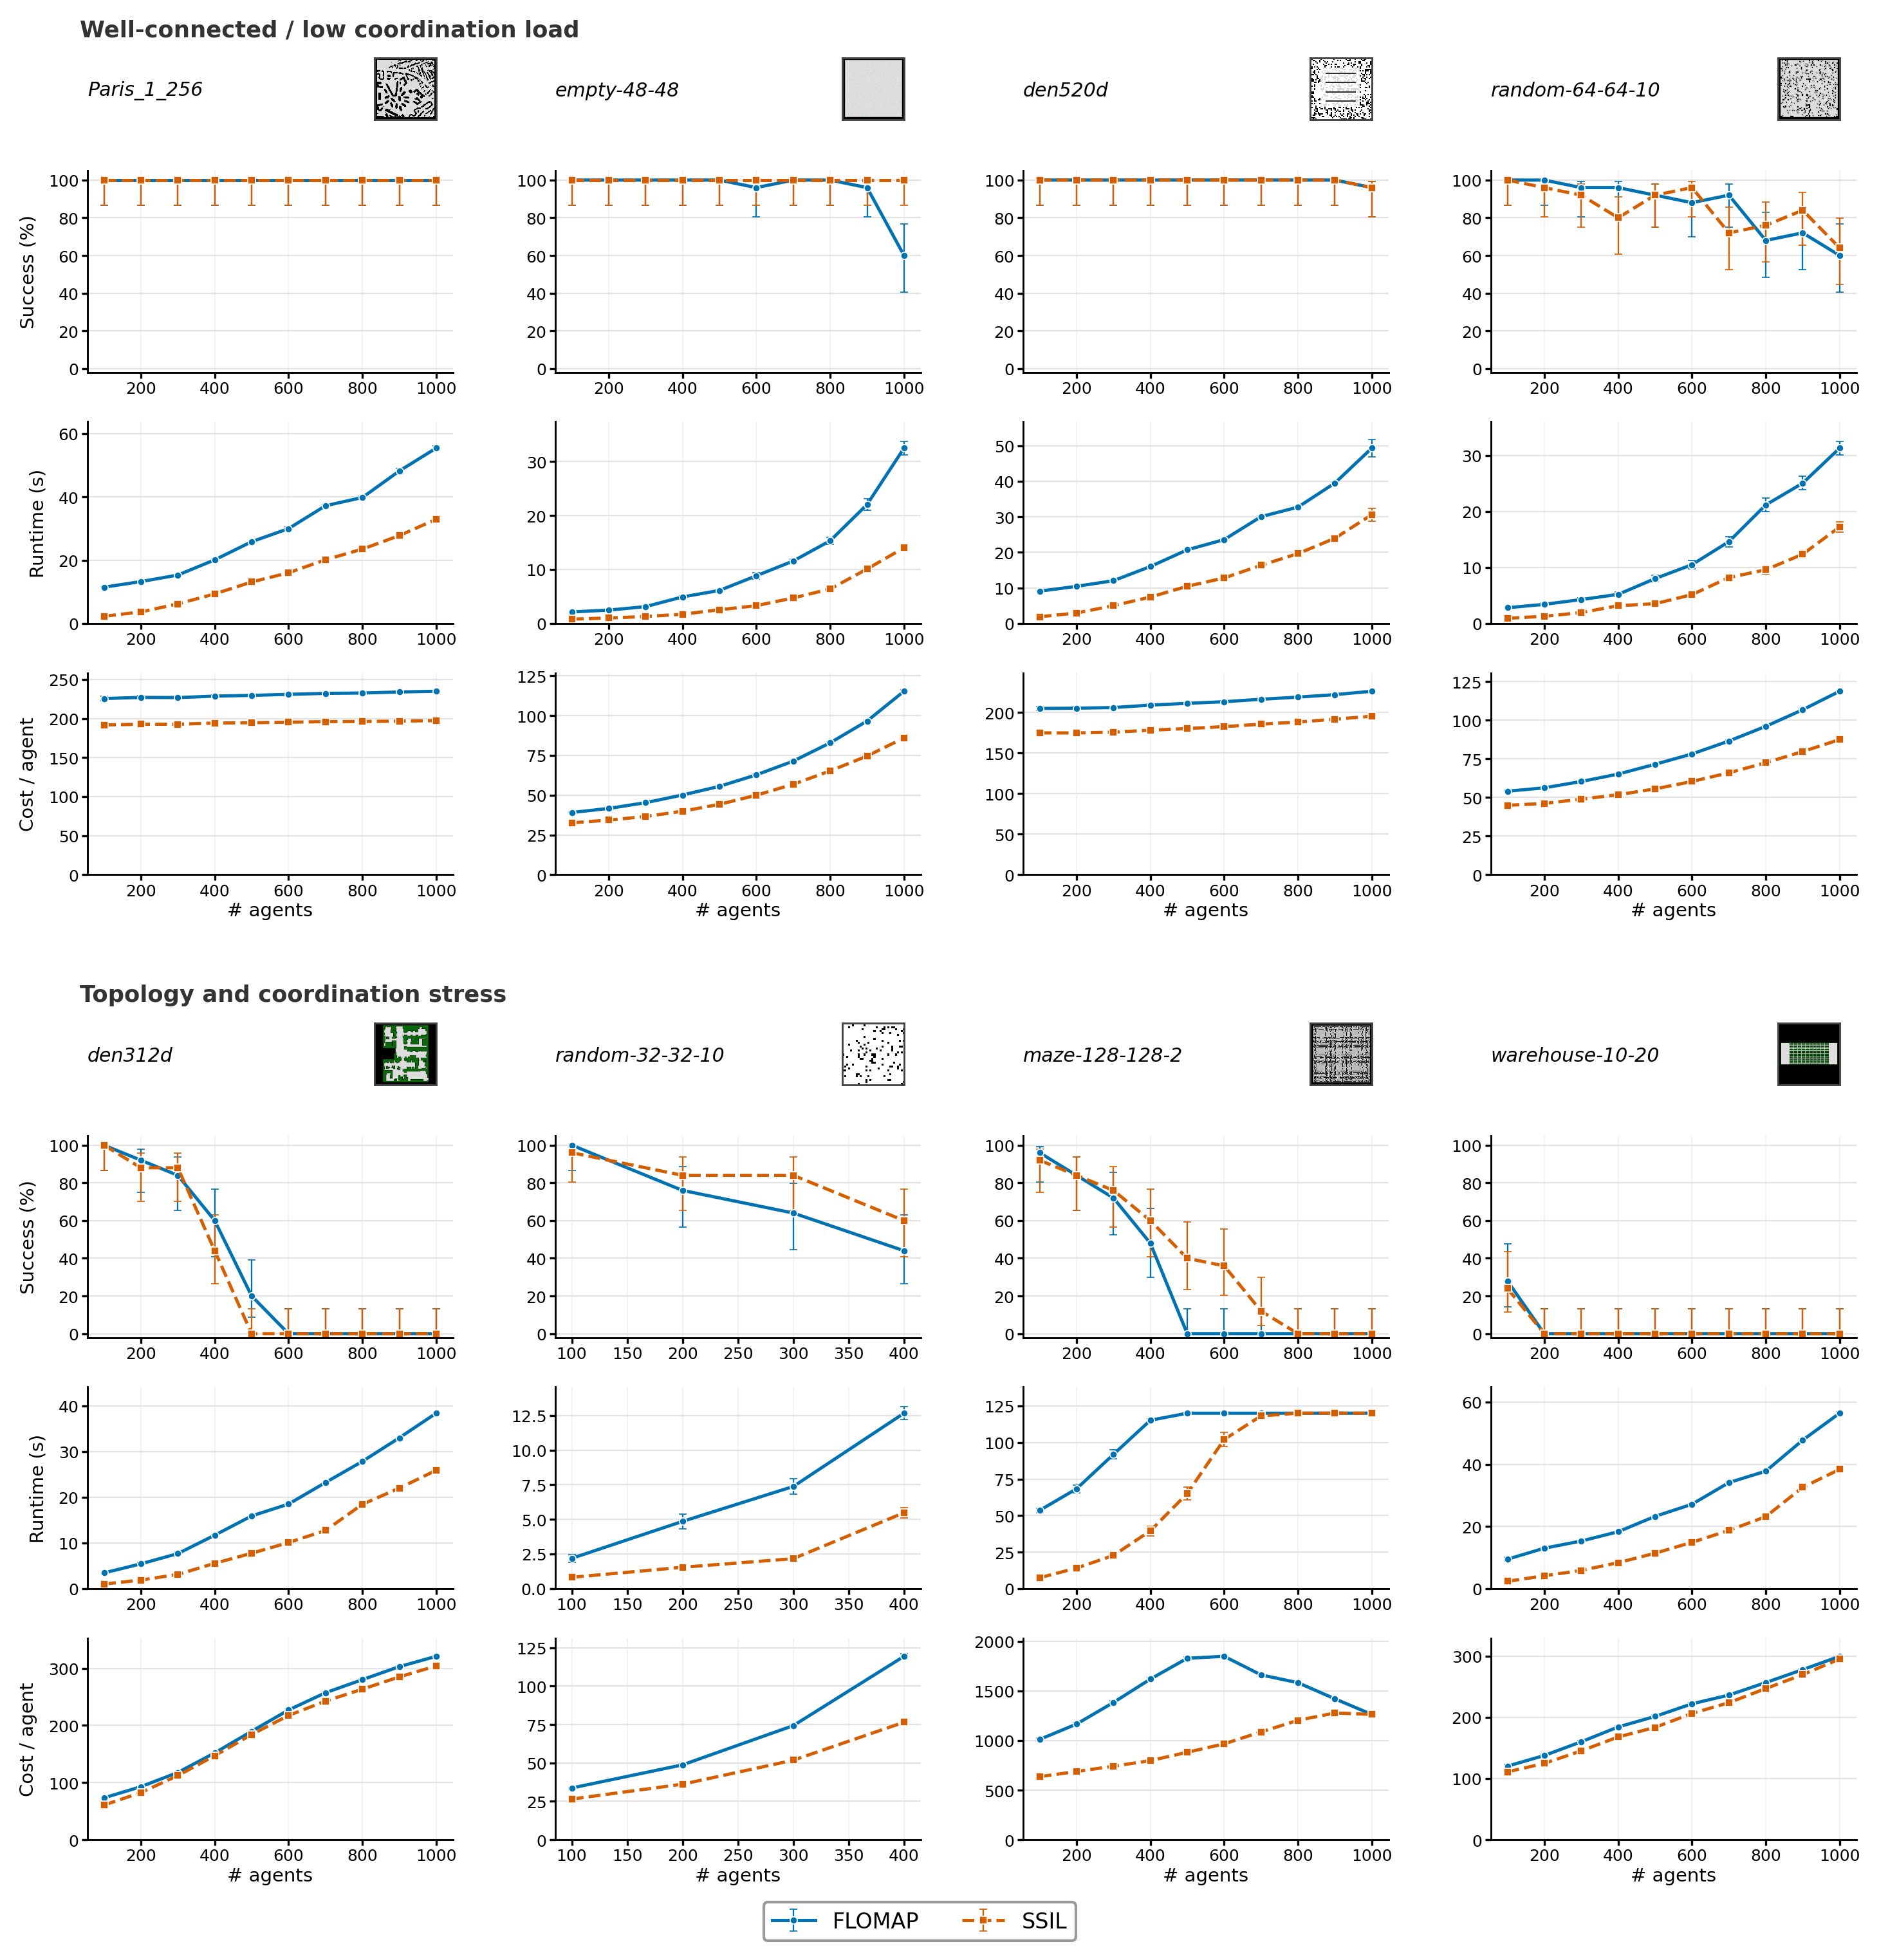
\includegraphics[width=0.98\textwidth,height=0.54\textheight,keepaspectratio]{figures/primary8_grouped_metric_panel.png}
\caption{Grouped learned-policy panel for the primary held-out evaluation.  Maps
are grouped by topology, with a small preview at the top of each column and
three metric rows: all-agent success, solution time, and path cost per agent.
Error bars show Wilson intervals for success and standard errors for runtime
and path cost; significance is evaluated by the paired tests in
Table~\ref{tab:coord-slices}, not by visual interval overlap.  The learned-policy gap is concentrated in dense random and maze bottleneck maps,
while open and well-connected maps are near parity or near ceiling.}
\label{fig:primary-grouped-panel}
\end{figure*}

Figure~\ref{fig:primary-grouped-panel} shows the learned-policy per-map trend.
On the primary held-out evaluation, FLOMAP reaches 100.00\% on
Paris\_1\_256, 99.60\% on den520d, 95.20\% on empty-48-48, and 86.40\% on
random-64-64-10.  It is weaker on maze-128-128-2 at 30.00\% and nearly at floor
on the warehouse map at 2.80\%.  SSIL has the clearest advantages on
random-32-32-10 and maze-128-128-2, both by 10.00 percentage points in the
aggregate table and especially at higher densities in
Fig.~\ref{fig:primary-grouped-panel}.

The cost and runtime rows add two qualifications.  First, lower path cost for
SSIL on several maps is consistent with its stronger direct action supervision,
but cost is not a substitute for success because incomplete runs can still be
assigned simulator costs.  Second, runtime is useful as implementation context
but not as a hardware-normalized algorithmic metric.  The extended topology
evaluation strengthens the baseline interpretation: current learned guidance
provides diagnostic insight, but it does not yet improve over
shortest-path preferences inside the same shield.
Across the density sweeps, the learned policies remain close on open and city
maps until high agent counts, whereas divergence appears earlier on dense random
and maze layouts.  In dense random and maze maps, divergence occurs at lower
agent counts, indicating earlier breakdown of learned coordination.  In
contrast, open maps maintain near parity until high densities, suggesting that
directional guidance is sufficient in lower-interaction regimes.  Overall, this
indicates that topology plays a significant role in addition to agent count when
one-step action supervision or heuristic preferences become more reliable than
the current FLOMAP velocity-to-action interface.

\subsection{Topology and Coordination Regimes}

\begin{figure*}[!tbp]
\centering
\resizebox{0.88\textwidth}{!}{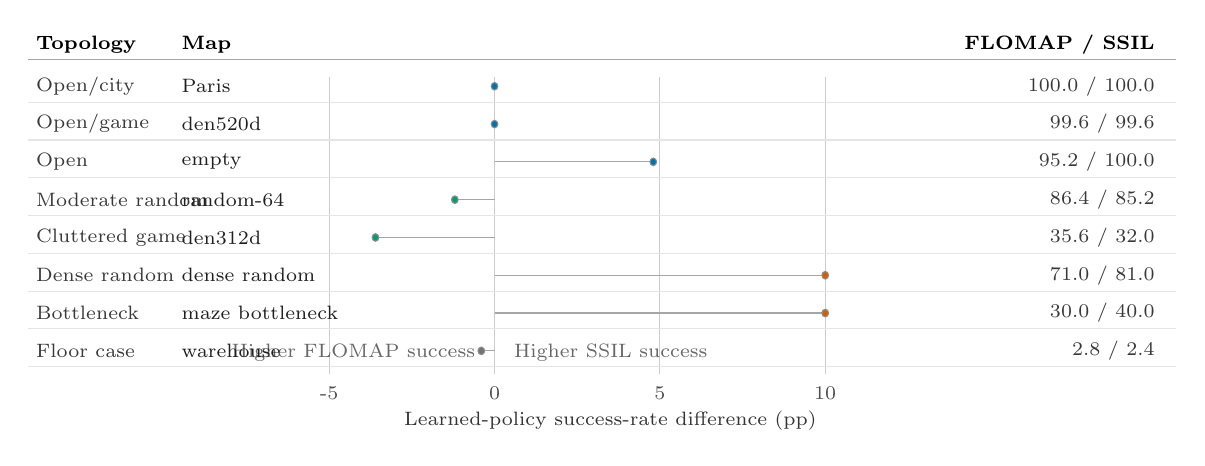
\begin{tikzpicture}[x=0.42cm,y=0.48cm]
\scriptsize
\node[anchor=west,font=\bfseries] at (-9.1,9.1) {Topology};
\node[anchor=west,font=\bfseries] at (-4.7,9.1) {Map};
\node[anchor=east,font=\bfseries] at (25.2,9.1) {FLOMAP / SSIL};
\draw[black!35] (-9.1,8.72) -- (25.6,8.72);
\draw[black!45] (5.00,0.45) -- (5.00,8.25);
\draw[black!20] (0.00,0.38) -- (0.00,8.25);\node[below,black!70] at (0.00,0.25) {-5};
\draw[black!20] (5.00,0.38) -- (5.00,8.25);\node[below,black!70] at (5.00,0.25) {0};
\draw[black!20] (10.00,0.38) -- (10.00,8.25);\node[below,black!70] at (10.00,0.25) {5};
\draw[black!20] (15.00,0.38) -- (15.00,8.25);\node[below,black!70] at (15.00,0.25) {10};
\node[below,black!80] at (8.50,-0.38) {Learned-policy success-rate difference (pp)};
\node[anchor=east,black!60] at (4.65,0.95) {Higher FLOMAP success};
\node[anchor=west,black!60] at (5.35,0.95) {Higher SSIL success};
\draw[black!10] (-9.1,7.58) -- (25.6,7.58);
\node[anchor=west,black!78] at (-9.1,8.00) {Open/city};
\node[anchor=west,black!88] at (-4.7,8.00) {Paris};
\draw[black!35,line width=0.45pt] (5.00,8.00) -- (5.00,8.00);
\filldraw[fill=oiBlue,draw=black!45] (5.00,8.00) circle[radius=0.10];
\node[anchor=east,black!78] at (25.2,8.00) {100.0 / 100.0};
\draw[black!10] (-9.1,6.58) -- (25.6,6.58);
\node[anchor=west,black!78] at (-9.1,7.00) {Open/game};
\node[anchor=west,black!88] at (-4.7,7.00) {den520d};
\draw[black!35,line width=0.45pt] (5.00,7.00) -- (5.00,7.00);
\filldraw[fill=oiBlue,draw=black!45] (5.00,7.00) circle[radius=0.10];
\node[anchor=east,black!78] at (25.2,7.00) {99.6 / 99.6};
\draw[black!10] (-9.1,5.58) -- (25.6,5.58);
\node[anchor=west,black!78] at (-9.1,6.00) {Open};
\node[anchor=west,black!88] at (-4.7,6.00) {empty};
\draw[black!35,line width=0.45pt] (5.00,6.00) -- (9.80,6.00);
\filldraw[fill=oiBlue,draw=black!45] (9.80,6.00) circle[radius=0.10];
\node[anchor=east,black!78] at (25.2,6.00) {95.2 / 100.0};
\draw[black!10] (-9.1,4.58) -- (25.6,4.58);
\node[anchor=west,black!78] at (-9.1,5.00) {Moderate random};
\node[anchor=west,black!88] at (-4.7,5.00) {random-64};
\draw[black!35,line width=0.45pt] (5.00,5.00) -- (3.80,5.00);
\filldraw[fill=oiBluishGreen,draw=black!45] (3.80,5.00) circle[radius=0.10];
\node[anchor=east,black!78] at (25.2,5.00) {86.4 / 85.2};
\draw[black!10] (-9.1,3.58) -- (25.6,3.58);
\node[anchor=west,black!78] at (-9.1,4.00) {Cluttered game};
\node[anchor=west,black!88] at (-4.7,4.00) {den312d};
\draw[black!35,line width=0.45pt] (5.00,4.00) -- (1.40,4.00);
\filldraw[fill=oiBluishGreen,draw=black!45] (1.40,4.00) circle[radius=0.10];
\node[anchor=east,black!78] at (25.2,4.00) {35.6 / 32.0};
\draw[black!10] (-9.1,2.58) -- (25.6,2.58);
\node[anchor=west,black!78] at (-9.1,3.00) {Dense random};
\node[anchor=west,black!88] at (-4.7,3.00) {dense random};
\draw[black!35,line width=0.45pt] (5.00,3.00) -- (15.00,3.00);
\filldraw[fill=oiVermillion,draw=black!45] (15.00,3.00) circle[radius=0.10];
\node[anchor=east,black!78] at (25.2,3.00) {71.0 / 81.0};
\draw[black!10] (-9.1,1.58) -- (25.6,1.58);
\node[anchor=west,black!78] at (-9.1,2.00) {Bottleneck};
\node[anchor=west,black!88] at (-4.7,2.00) {maze bottleneck};
\draw[black!35,line width=0.45pt] (5.00,2.00) -- (15.00,2.00);
\filldraw[fill=oiVermillion,draw=black!45] (15.00,2.00) circle[radius=0.10];
\node[anchor=east,black!78] at (25.2,2.00) {30.0 / 40.0};
\draw[black!10] (-9.1,0.58) -- (25.6,0.58);
\node[anchor=west,black!78] at (-9.1,1.00) {Floor case};
\node[anchor=west,black!88] at (-4.7,1.00) {warehouse};
\draw[black!35,line width=0.45pt] (5.00,1.00) -- (4.60,1.00);
\filldraw[fill=black!55,draw=black!45] (4.60,1.00) circle[radius=0.10];
\node[anchor=east,black!78] at (25.2,1.00) {2.8 / 2.4};
\end{tikzpicture}
}
\caption{Topology-stratified learned-policy success gap on the primary held-out
evaluation.  Bars show the success-rate difference between SSIL and the
FLOMAP policy; positive values indicate higher SSIL success and negative
values indicate higher FLOMAP success.  Dense random and bottleneck maps
account for the largest positive gaps, while well-connected maps remain close to
parity.  These results support a
topology-specific interpretation of the learned-policy residual gap.}
\label{fig:topology-regime}
\end{figure*}

\begin{table}[!tbp]
\centering
\caption{Primary held-out success with and without coordination-heavy
maps.  The final column reports paired McNemar tests on matched evaluation
instances.}
\label{tab:coord-slices}
\scriptsize
\setlength{\tabcolsep}{4pt}
\begin{tabular}{p{0.34\linewidth}p{0.16\linewidth}p{0.16\linewidth}p{0.14\linewidth}p{0.12\linewidth}}
\toprule
Slice & FLOMAP & SSIL & Gap (pp) & McNemar p \\
\midrule
Full primary held-out evaluation & 64.59 (1195/1850) & 66.43 (1229/1850) & SSIL +1.84 & 0.0039 \\
Coordination stress maps & 41.71 (146/350) & 51.71 (181/350) & SSIL +10.00 & $<$0.001 \\
Dense random map & 71.00 (71/100) & 81.00 (81/100) & SSIL +10.00 & 0.064 \\
Maze bottleneck map & 30.00 (75/250) & 40.00 (100/250) & SSIL +10.00 & $<$0.001 \\
Excluding coordination stress maps & 69.93 (1049/1500) & 69.87 (1048/1500) & FLOMAP +0.06 & 1.000 \\
Excluding stress and floor-case maps & 83.36 (1042/1250) & 83.36 (1042/1250) & 0.00 & 1.000 \\
\bottomrule
\end{tabular}

\end{table}

The topology view in Fig.~\ref{fig:topology-regime} and the slice analysis in
Table~\ref{tab:coord-slices} isolate a learned-policy comparison.  On the full
primary held-out evaluation, SSIL is ahead of FLOMAP by 1.84 percentage
points, and the paired McNemar test is significant ($p=0.0039$).  On the
coordination-stress slice consisting of dense random and maze bottleneck maps,
the gap grows to 10.00 percentage points ($p<0.001$).  Removing those two maps
leaves only a 0.06 percentage-point difference: 69.93\% versus 69.87\%, with no
significant paired difference ($p=1.0$).
Removing the warehouse map as well gives an exact tie at 83.36\%.

These results support a topology-dependent learned-policy interpretation: the
FLOMAP policy is close to SSIL when a smooth directional preference plus
CS-PIBT shielding is
enough, but SSIL appears better aligned with tasks that require
explicit wait and yield decisions.  This observation should be read as
topology-specific evidence, not as evidence that flow-based policies cannot
learn coordination.  The BD-PIBT result changes the broader interpretation: strong
backward-Dijkstra preferences plus CS-PIBT already encode an effective
goal-directed and coordination-compatible prior under this protocol, so learned
guidance must improve over that baseline as well as over learned alternatives.

\section{Ablations}

Table~\ref{tab:ablation} summarizes qualitative conclusions from the
quantitative ablation results reported in this section.

\begin{table*}[!tbp]
\centering
\caption{Ablation inference matrix.  The table emphasizes what each
intervention supports, rather than ranking variants by a single success number.}
\label{tab:ablation}
\scriptsize
\setlength{\tabcolsep}{4pt}
\begin{tabular}{p{0.21\linewidth}p{0.20\linewidth}p{0.20\linewidth}p{0.31\linewidth}}
\toprule
Intervention & Targeted topology & Broader evaluation & Supported inference \\
\midrule
Action-interface alignment & Improved with state alignment & Below BD-PIBT and FLOMAP & The action interface is sensitive to the state distribution seen at inference; adding an action head alone is insufficient. \\
Discrete-primary supervision & Coordination target improved & Below BD-PIBT overall & Discrete action labels can help coordination-heavy behavior, but stronger discrete pressure can over-specialize. \\
Coordination-focused data & Target topology improved & Below BD-PIBT overall & Topology-targeted data can move the desired slice; the data mixture and stopping rule still limit out-of-distribution transfer. \\
Hybrid action policy & No robust target gain & Below BD-PIBT and FLOMAP & The hybrid head did not replace the velocity policy as the most robust interface. \\
Reduced-capacity hybrid & No clear target advantage & Below BD-PIBT and FLOMAP & Capacity reduction did not explain the coordination-heavy gap. \\
\bottomrule
\end{tabular}

\end{table*}

\subsection{Action-Interface Alignment}

The first action-head experiments exposed a train/inference mismatch.  The
original direct action head achieved 0.00\% in the short diagnostic setting
(Table~\ref{tab:eval-settings}).  Conditioning the head on the integrated flow
state improved the same setting to 43.48\%, whereas zero-state conditioning
remained at 0.00\%.  This suggests that the action head was sensitive to the
state distribution it saw at inference.

An action-state variant improved to 69.57\% in the short diagnostic setting and
62.70\% under the medium diagnostic setting.  Performance
therefore improved after aligning the action-head training and inference states,
but the variant still underperformed relative to FLOMAP on the
more comparable benchmark scale and did not surpass BD-PIBT in the primary
comparison.  This supports an interface-alignment interpretation:
action-state consistency matters, while the shared trunk remains optimized
primarily for continuous velocity prediction.

\subsection{Discrete-Primary Supervision}

A reduced-capacity hybrid reached 60.87\% in the short diagnostic setting
and underperformed relative to FLOMAP.  A stronger
discrete-primary objective with higher action-loss weight reached a lower
validation loss than the smaller hybrid.  Across action-selection thresholds
0.15, 0.20, 0.30, and 0.50, the
short diagnostic setting reached 60.87\%, 60.87\%, 56.52\%, and 65.22\%,
respectively; the dense-random map reached 100\% at threshold 0.30 in that
setting.

The medium diagnostic setting clarified the trade-off.  At threshold 0.30,
the discrete-primary model reached 60.00\% overall and 75\% on the dense-random
map.  At threshold 0.50, it reached 61.08\% overall and 60\% on the same map.
The results suggest that stronger discrete supervision can
improve a dense coordination target, but the same supervision pressure appears
to reduce broader
generalization and did not surpass BD-PIBT overall.  They do not show that
discrete supervision is always better or that flow supervision is incapable of
coordination.

\subsection{Coordination-Focused Data}

The coordination-focused data experiments tested whether additional dense
coordination examples improve FLOMAP.  The full preprocessed
dataset was reduced to a targeted coordination subset to keep preprocessing
tractable.  This setup is best interpreted as an
in-distribution topology probe for dense coordination behavior, while the full
primary held-out evaluation measures broader transfer.

The strict flow-only control reached 62.43\% under the medium diagnostic
setting at the earliest evaluated model selection point, with dense-random success at
70\%.  At two later evaluated points, broad diagnostic success declined to
61.62\% and 60.54\%,
with dense-random success dropping to 65\% and 60\%.  The corresponding hybrid
variants reached 63.78\%, 64.59\%, and 63.78\% across the same selections, but
their dense-random values stayed at 55\%, 55\%, and 60\%.

The final hybrid action-policy evaluation reached 62.49\% overall,
including 58\% on the dense-random map and 69.20\% on the larger random map.  It
underperformed relative to the primary FLOMAP result of 64.59\%.  The
coordination-focused data results are therefore diagnostic: additional
coordination data can improve specific dense-map metrics, but the current
mixture and objectives did not change the final method ranking and did not
improve over BD-PIBT in the final shared-protocol comparisons.

\section{Discussion}

The results support four conclusions.  First, BD-guided CS-PIBT achieves the
best performance in this evaluation.  It ties SSIL on the primary
held-out evaluation and exceeds both learned methods on the extended topology
evaluation.  Second, continuous
FLOMAP guidance is a viable learned action-prior interface for shielded
MAPF, but it has not demonstrated improvement over BD-guided preferences.
Third, the FLOMAP versus SSIL gap is concentrated in maps where success
depends on precise waiting, yielding, and bottleneck negotiation.  Fourth,
direct action-head and hybrid variants improved some diagnostics but did not
robustly surpass FLOMAP or BD-PIBT in the final comparison.

These results should not be interpreted as a broad performance claim for
FLOMAP or as evidence that flow matching is incapable of coordination.
They also do not isolate a single causal mechanism, because
the objective, training distribution, architecture, data mixture, and
velocity-to-action conversion are coupled.

A key implication is that learned guidance must improve over a strong
preference generator already available to CS-PIBT.  Backward-Dijkstra rankings
provide stable goal-directed one-step preferences, and CS-PIBT supplies priority
updates and collision resolution around those preferences.  The current
FLOMAP velocity-to-action interface may distort useful short-horizon routing or wait behavior in some
regimes, especially when continuous velocities are discretized into a ranked
action list.  The results support this interpretation.

One explanation is interface alignment.  SSIL is trained from the
start on the same five-way action decision that CS-PIBT consumes.  FLOMAP
is trained to predict continuous velocities and then maps those velocities into
discrete preferences.  That mapping is natural when the correct behavior is
mostly directional.  It is less expressive when the key decision is whether to
wait, yield, or claim a narrow passage at exactly the right time step.  The
wait-threshold rule addresses the most obvious zero-vector issue, but it
remains a manually specified bridge between a continuous output and a discrete
shield.

The dot-product action interface was chosen to preserve the geometric semantics
of the learned velocity field rather than adding a learned projection that would
make the method closer to a discrete classifier.  Its limitation is that it
collapses speed, uncertainty, and interaction priority into a single ranked action
list, which limits representation of discrete coordination decisions such as
yielding and waiting.  Varying the wait threshold would trade off premature motion against
excessive waiting: a low threshold can miss yield states, while a high threshold
can suppress progress.  The current experiments support treating this
conversion as an interface sensitivity rather than attributing the topology gap
to the wait threshold alone.

The runtime results expose a second trade-off.  FLOMAP requires three Euler
steps for each of three consensus samples before CS-PIBT can construct action
preferences, whereas SSIL emits discrete logits in a single classifier pass and
BD-PIBT ranks actions directly from distance fields.  This additional continuous
simulation cost is visible in the end-to-end runtimes in
Table~\ref{tab:overall}.  Future learned
flow policies therefore need to improve either success, runtime, or both to
justify the extra interface cost over discrete or heuristic preference
generators.

The action-head and hybrid ablations help refine the learned-policy
interpretation.  The
state-aligned action interface shows that inference distribution matters.  The
discrete-primary hybrid shows that stronger action supervision can improve a
dense-random target in some settings.  The flow-only control with
coordination-focused data shows that dense coordination examples can improve
FLOMAP behavior on a target topology.  Because none of these variants
improves the final ranking against BD-PIBT, the remaining challenge
is a coupled representation, objective, data-balance, and shield-interface
problem.

\section{Limitations}

The main modeling limitation is the velocity-to-action discretization step.
The learned policy predicts a continuous vector field, but the shield consumes a
ranked list of discrete grid actions.  This interface is natural when the
correct behavior is mostly directional, but it is less direct when success
depends on waiting, yielding, or negotiating a narrow passage at a precise
time step.

A second limitation is that the current learned policy has not demonstrated
improvement over BD-guided CS-PIBT.  This limits claims about learned guidance
as an overall replacement for heuristic preferences.  The evaluation remains
useful because it isolates the preference generator under a shared shield and
therefore identifies what the learned model must improve.

Another limitation is performance on dense coordination and bottleneck maps.
CS-PIBT guarantees one-step collision avoidance, but it does not provide a
global completion guarantee and can require strong preference signals to avoid
livelock or livelock-like behavior in constrained topologies.  A third limitation is
evaluation scale: short diagnostic evaluations were useful for screening
variants, but they sometimes overestimated performance relative to larger
diagnostic evaluations.  The final conclusions are therefore based on the larger
comparisons and topology-level slices.

All-agent success is also a stringent metric.  It can obscure partial progress,
while mean agents at goal can obscure a small number of unresolved blocking
agents.  Both metrics are therefore needed.

Flow integration and consensus sampling also increase runtime relative to a
direct classifier.  The wait threshold is a hand-tuned conversion rule rather
than a learned coordination policy, which may limit adaptation across map
topologies and density regimes.  We therefore avoid attributing the topology
gap to the wait threshold alone.

\section{Future Work}

Future work should prioritize improving the preference generator relative to
BD-PIBT rather than only adding capacity.  Promising directions include learning
residuals over backward-Dijkstra preferences, hybrid BD-plus-flow action
rankings, learned wait calibration, uncertainty-aware action ranking, and
imitation targets that preserve shortest-path monotonicity while adding
coordination-specific corrections.  A second direction is data selection:
coordination-heavy examples should be sampled deliberately, but with mixture
weights that preserve performance on large city, open, and random-64 maps.
Third, evaluation should separate full benchmark performance from diagnostic
slices so that dense-map gains are not mistaken for broad improvements.  Future
learned policies should include BD-PIBT as a required baseline under the same
shielded protocol.  Finally, stronger shield variants or lookahead mechanisms,
including LaCAM-style components, may be needed when one-step conflict
resolution cannot negotiate long bottlenecks.

\section{Conclusion}

FLOMAP demonstrates that a rectified-flow GNN can provide learned
velocity guidance for CS-PIBT-shielded MAPF.  The primary FLOMAP policy trails
SSIL on the full primary held-out evaluation by a statistically resolved margin
($p=0.0039$), but the non-coordination-heavy learned-policy slices are not
significantly different under a paired McNemar test ($p=1.0$).  The
completed comparison places BD-PIBT ahead overall, with the highest extended
topology success and highest mean agents at goal.  The
contribution is therefore a measured experimental analysis of learned flow
guidance under a shared CS-PIBT shield, rather than an overall performance
claim.  The ablations identify interface and data-mixture factors,
while the BD-PIBT result
clarifies that shortest-path heuristic preferences with CS-PIBT form a strong
evaluation baseline for learned shielded MAPF.

\appendices

\section{Additional Per-Map Results}
\vspace{0.25em}

\subsection{Primary Held-Out Evaluation}
\captionof{table}{Primary held-out learned-policy per-map success.}
\label{tab:appendix-primary-per-map}
\vspace{0.25em}

\noindent\resizebox{\columnwidth}{!}{\input{tables/primary8_per_map_success.tex}}

\vspace{0.65em}
\subsection{Extended Topology Evaluation}
\captionof{table}{Extended topology learned-policy per-map success.}
\label{tab:appendix-extended-per-map}
\vspace{0.25em}

\noindent\resizebox{\columnwidth}{!}{\scriptsize
\setlength{\tabcolsep}{4pt}
\begin{tabular}{lrrr}
\toprule
Map & FLOMAP & SSIL & Gap (pp) \\
\midrule
Berlin\_1\_256 & 99.60 & 100.00 & SSIL +0.40 \\
Paris\_1\_256 & 100.00 & 100.00 & 0.00 \\
den312d & 35.60 & 32.00 & FLOMAP +3.60 \\
empty-32-32 & 80.80 & 100.00 & SSIL +19.20 \\
empty-48-48 & 95.20 & 100.00 & SSIL +4.80 \\
maze-128-128-2 & 30.00 & 42.00 & SSIL +12.00 \\
maze-32-32-4 & 21.33 & 14.67 & FLOMAP +6.66 \\
random-64-64-10 & 86.40 & 85.20 & FLOMAP +1.20 \\
random-64-64-20 & 40.80 & 42.00 & SSIL +1.20 \\
room-64-64-16 & 21.20 & 27.20 & SSIL +6.00 \\
warehouse-10-20-10-2-1 & 2.80 & 2.40 & FLOMAP +0.40 \\
warehouse-20-40-10-2-1 & 14.80 & 11.20 & FLOMAP +3.60 \\
\bottomrule
\end{tabular}
}

\section{Additional Data Summary}
\vspace{0.35em}

\captionof{table}{Training and coordination-focused data summary.}
\label{tab:appendix-data-summary}
\vspace{0.25em}

\noindent\scriptsize
\setlength{\tabcolsep}{3pt}
\begin{tabular}{lrp{0.43\linewidth}}
\toprule
Data source & Count & Note \\
\midrule
Base demonstration pool & 1,169,520 samples & Main training source. \\
Targeted coordination subset & 7 maps; 28,935 samples & Used for dense and bottlenecked topology ablations. \\
\bottomrule
\end{tabular}
\normalsize

\balance
\bibliographystyle{IEEEtran}
\bibliography{references}

\end{document}
